\section{Roles en Kanban}

A diferencia de otras metodologías ágiles como Scrum, Kanban no define de manera explícita roles formales o jerarquías dentro del equipo. Esta característica responde a su filosofía de mínima interrupción de los procesos existentes, enfocándose en la mejora continua a partir del flujo de trabajo actual.

\subsection{Enfoque general de los roles en Kanban}

En Kanban, todos los miembros del equipo son responsables del flujo de trabajo. No obstante, en la práctica, algunos roles pueden emerger de manera natural para facilitar la gestión y mejora del sistema. Estos roles, aunque no impuestos por la metodología, pueden aportar claridad, liderazgo y soporte al proceso.

\subsection{Roles emergentes comunes}
\begin{figure}[H]
    \centering
    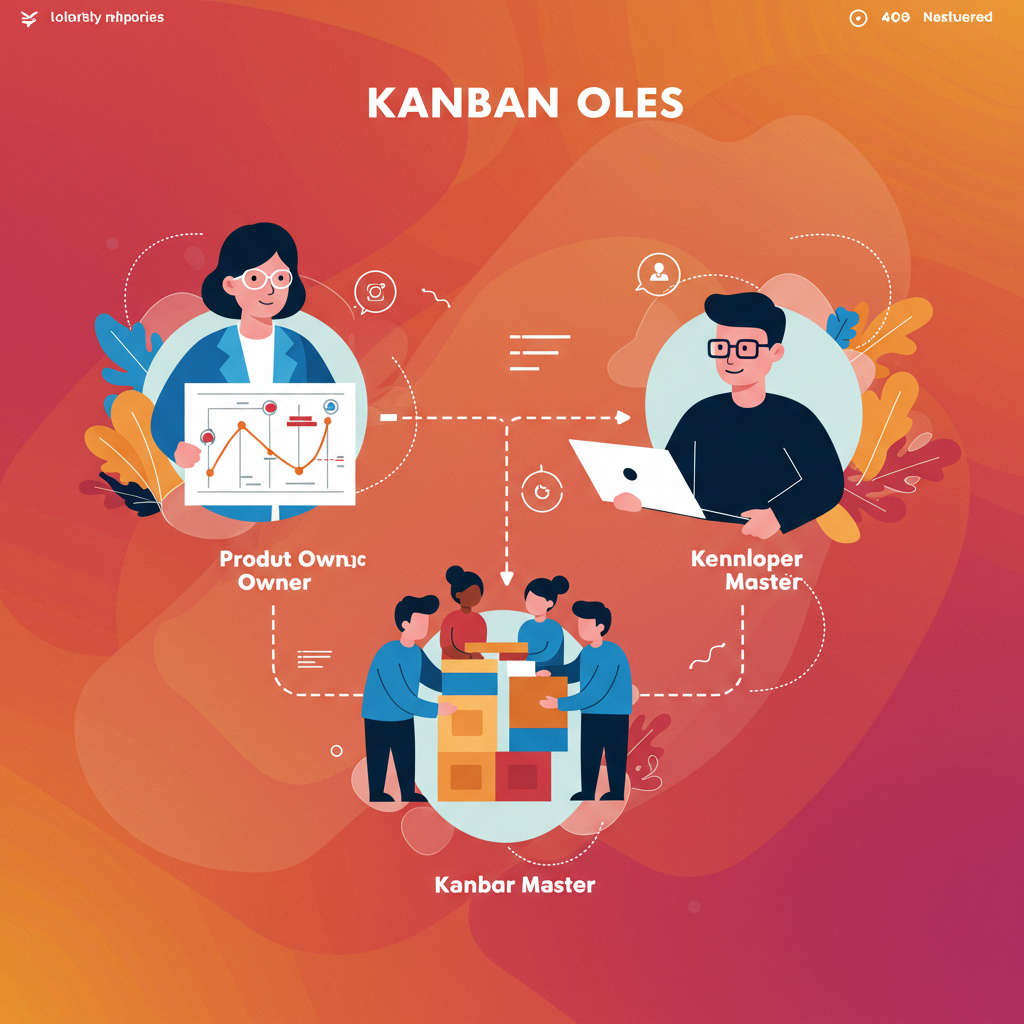
\includegraphics[width=0.6\textwidth]{assets/images/roles-kanban.png}
    \caption{Roles emergentes en Kanban y su relación con el flujo de trabajo}
    \label{fig:roles-kanban}
\end{figure}

A continuación, se describen los roles más comunes que suelen encontrarse en equipos que adoptan Kanban:

\subsubsection{Equipo de trabajo (Team Members)}

Son los responsables de ejecutar las tareas visibles en el tablero. Esto incluye desarrolladores, analistas, diseñadores u otros especialistas según el contexto del equipo. Cada miembro contribuye al cumplimiento de los objetivos colectivos y comparte la responsabilidad de mantener el flujo de trabajo en movimiento.

\subsubsection{Facilitador o Service Delivery Manager (SDM)}

Aunque no es un rol obligatorio, muchas organizaciones designan a una persona encargada de observar y optimizar el flujo. Su función se asemeja en cierta medida al \textit{Scrum Master}, aunque con un enfoque más operativo:
\begin{itemize}
    \item Detectar cuellos de botella
    \item Asegurar que los límites WIP se respeten
    \item Facilitar reuniones de mejora continua
    \item Promover la colaboración entre las partes interesadas
\end{itemize}

\subsubsection{Product Owner o Request Manager}

Cuando se trabaja en entornos con múltiples solicitudes externas, este rol emerge como intermediario entre los stakeholders y el equipo. Se encarga de priorizar las tareas, clarificar requerimientos y asegurar que el trabajo refleje el valor esperado por el cliente.

\subsection{Comparación con Scrum}

\begin{longtable}{|p{5cm}|p{5cm}|}
\hline
\textbf{Scrum} & \textbf{Kanban} \\
\hline
Scrum Master: facilitador y guía del proceso & Puede haber un Facilitador, pero no es obligatorio \\
\hline
Product Owner: responsable del valor del producto & Puede existir un Request Manager que prioriza el trabajo \\
\hline
Equipo de desarrollo: multifuncional y autogestionado & Equipo responsable del flujo, sin roles estrictos \\
\hline
Roles definidos y requeridos & Roles flexibles y emergentes según necesidad \\
\hline
\end{longtable}

\subsection{Responsabilidad compartida}

Una característica clave de Kanban es que todos los integrantes comparten la responsabilidad sobre:
\begin{itemize}
    \item El cumplimiento de los límites WIP
    \item La calidad del trabajo entregado
    \item La identificación de oportunidades de mejora
    \item La documentación de políticas y cambios en el flujo
\end{itemize}

Esto refuerza una cultura de colaboración constante y evolución adaptativa, que busca la eficiencia más allá de los roles individuales.

